\documentclass[]{article}
\usepackage{lmodern}
\usepackage{amssymb,amsmath}
\usepackage{ifxetex,ifluatex}
\usepackage{fixltx2e} % provides \textsubscript
\ifnum 0\ifxetex 1\fi\ifluatex 1\fi=0 % if pdftex
  \usepackage[T1]{fontenc}
  \usepackage[utf8]{inputenc}
\else % if luatex or xelatex
  \ifxetex
    \usepackage{mathspec}
  \else
    \usepackage{fontspec}
  \fi
  \defaultfontfeatures{Ligatures=TeX,Scale=MatchLowercase}
\fi
% use upquote if available, for straight quotes in verbatim environments
\IfFileExists{upquote.sty}{\usepackage{upquote}}{}
% use microtype if available
\IfFileExists{microtype.sty}{%
\usepackage{microtype}
\UseMicrotypeSet[protrusion]{basicmath} % disable protrusion for tt fonts
}{}
\usepackage[margin=1in]{geometry}
\usepackage{hyperref}
\hypersetup{unicode=true,
            pdftitle={DDS Analytics},
            pdfauthor={Authors: Daniel Davieau, Lakeitra Webb, Emil Ramos},
            pdfborder={0 0 0},
            breaklinks=true}
\urlstyle{same}  % don't use monospace font for urls
\usepackage{graphicx,grffile}
\makeatletter
\def\maxwidth{\ifdim\Gin@nat@width>\linewidth\linewidth\else\Gin@nat@width\fi}
\def\maxheight{\ifdim\Gin@nat@height>\textheight\textheight\else\Gin@nat@height\fi}
\makeatother
% Scale images if necessary, so that they will not overflow the page
% margins by default, and it is still possible to overwrite the defaults
% using explicit options in \includegraphics[width, height, ...]{}
\setkeys{Gin}{width=\maxwidth,height=\maxheight,keepaspectratio}
\IfFileExists{parskip.sty}{%
\usepackage{parskip}
}{% else
\setlength{\parindent}{0pt}
\setlength{\parskip}{6pt plus 2pt minus 1pt}
}
\setlength{\emergencystretch}{3em}  % prevent overfull lines
\providecommand{\tightlist}{%
  \setlength{\itemsep}{0pt}\setlength{\parskip}{0pt}}
\setcounter{secnumdepth}{0}
% Redefines (sub)paragraphs to behave more like sections
\ifx\paragraph\undefined\else
\let\oldparagraph\paragraph
\renewcommand{\paragraph}[1]{\oldparagraph{#1}\mbox{}}
\fi
\ifx\subparagraph\undefined\else
\let\oldsubparagraph\subparagraph
\renewcommand{\subparagraph}[1]{\oldsubparagraph{#1}\mbox{}}
\fi

%%% Use protect on footnotes to avoid problems with footnotes in titles
\let\rmarkdownfootnote\footnote%
\def\footnote{\protect\rmarkdownfootnote}

%%% Change title format to be more compact
\usepackage{titling}

% Create subtitle command for use in maketitle
\newcommand{\subtitle}[1]{
  \posttitle{
    \begin{center}\large#1\end{center}
    }
}

\setlength{\droptitle}{-2em}
  \title{DDS Analytics}
  \pretitle{\vspace{\droptitle}\centering\huge}
  \posttitle{\par}
  \author{Authors: Daniel Davieau, Lakeitra Webb, Emil Ramos}
  \preauthor{\centering\large\emph}
  \postauthor{\par}
  \predate{\centering\large\emph}
  \postdate{\par}
  \date{April 24, 2018}

\usepackage{booktabs}
\usepackage{longtable}
\usepackage{array}
\usepackage{multirow}
\usepackage[table]{xcolor}
\usepackage{wrapfig}
\usepackage{float}
\usepackage{colortbl}
\usepackage{pdflscape}
\usepackage{tabu}
\usepackage{threeparttable}
\usepackage{threeparttablex}
\usepackage[normalem]{ulem}
\usepackage{makecell}

\begin{document}
\maketitle

\subsection{Business Objective}\label{business-objective}

The leadership has identified predicting employee turnover as its first
application of data science for talent management. Before investing in
the project they would like an analysis of existing employee data.

\subsection{Data}\label{data}

Data was provided by the client in form of a .csv file
``CaseStudy2-data.xlsx''.

\paragraph{Basic Statistics}\label{basic-statistics}

The data includes a total of 1470 current and terminated employee
records with 35 variables.

Data Records

Observations

1470

Variables

35

Summary of measures included in the data:

DailyRate

Number of Companies Worked

Years at Company

Years with Manager

Distance From Home

Percent Salary Hike

Years in Current Role

Min.

102.0000

0.000000

0.000000

0.000000

1.000000

11.00000

0.000000

1st Qu.

465.0000

1.000000

3.000000

2.000000

2.000000

12.00000

2.000000

Median

802.0000

2.000000

5.000000

3.000000

7.000000

14.00000

3.000000

Mean

802.4857

2.693197

7.008163

4.123129

9.192517

15.20952

4.229252

3rd Qu.

1157.0000

4.000000

9.000000

7.000000

14.000000

18.00000

7.000000

Max.

1499.0000

9.000000

40.000000

17.000000

29.000000

25.00000

18.000000

\subsection{Methodology}\label{methodology}

Attrition is the central theme of this analysis. We interpreted the
value ``Yes'' in the data provided under attrition as an indicator that
the employee is terminated.

We categorized each record as ``Current'' or ``Terminated'' and look for
patterns in the variables that may explain why employees become
terminated.

\emph{\textbf{Current} meaning currently employed by the firm.}\\
\emph{\textbf{Terminated} meaning left the firm (voluntarily or
non-voluntarily)}

\begin{center}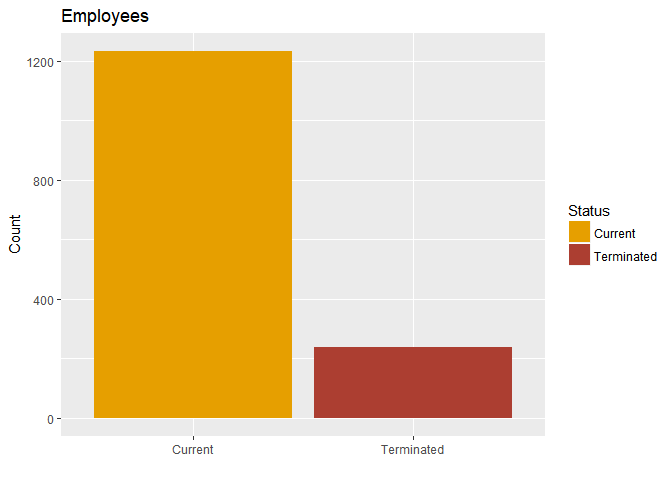
\includegraphics{DDSAnalytics_files/figure-latex/unnamed-chunk-4-1} \end{center}

As requested employees under the age of 18 have been excluded from this
analsyis. The table below shows the youngest age record included in the
data:

Youngest Age Record

18

\paragraph{Distributions}\label{distributions}

The following are the distributions of employees by various measures.

\begin{center}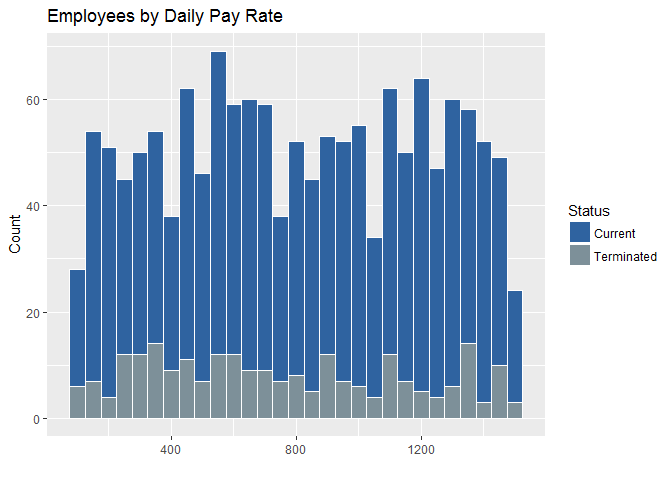
\includegraphics{DDSAnalytics_files/figure-latex/unnamed-chunk-7-1} \end{center}

\begin{center}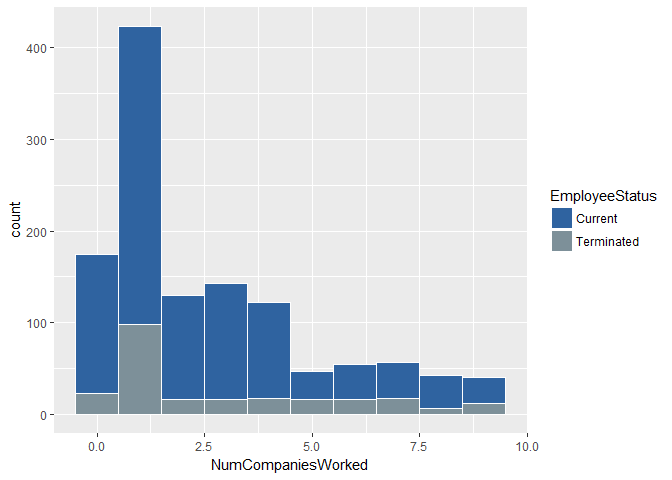
\includegraphics{DDSAnalytics_files/figure-latex/unnamed-chunk-7-2} \end{center}

\begin{center}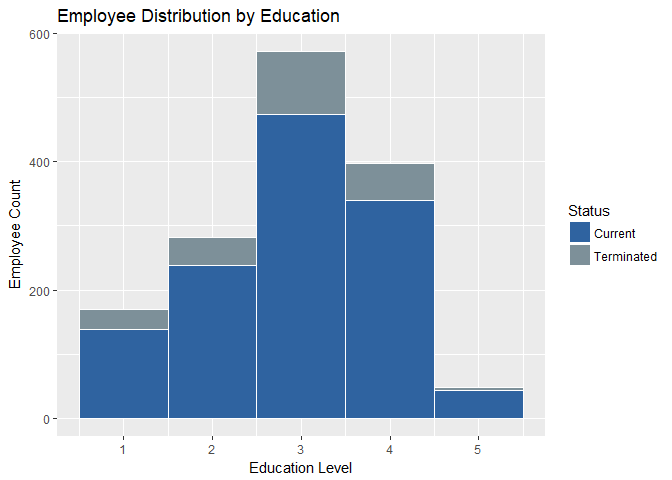
\includegraphics{DDSAnalytics_files/figure-latex/unnamed-chunk-8-1} \end{center}

\paragraph{Frequencies}\label{frequencies}

The following are frequencies by Gender and Job Roles

\begin{center}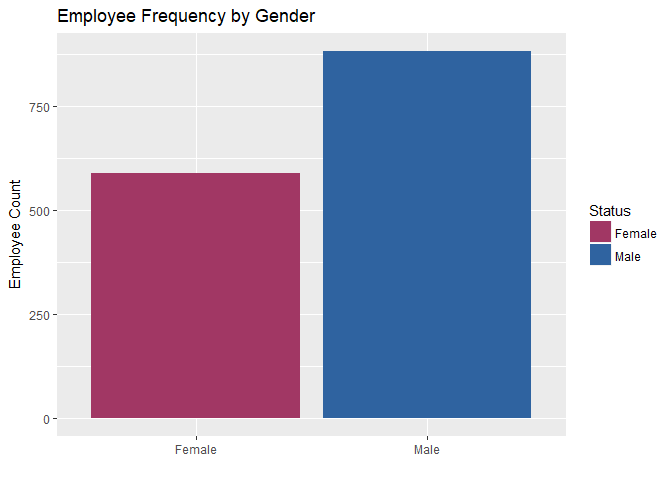
\includegraphics{DDSAnalytics_files/figure-latex/unnamed-chunk-9-1} \end{center}

\begin{center}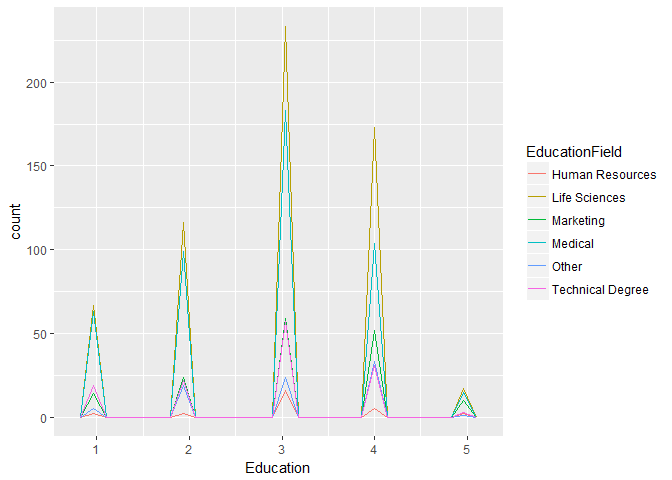
\includegraphics{DDSAnalytics_files/figure-latex/unnamed-chunk-9-2} \end{center}

As requested we have captured the counts of management positions in the
table below:

Count

Sales Executives

326

Manufacturing Directors

145

Managers

102

Research Directors

80

\paragraph{Is there a relationship between Age and
Income?}\label{is-there-a-relationship-between-age-and-income}

There's no apparent relationship between Age and Income. The plot below
shows a very slight upward incline as age increases but is relatively
insignificant.

\begin{center}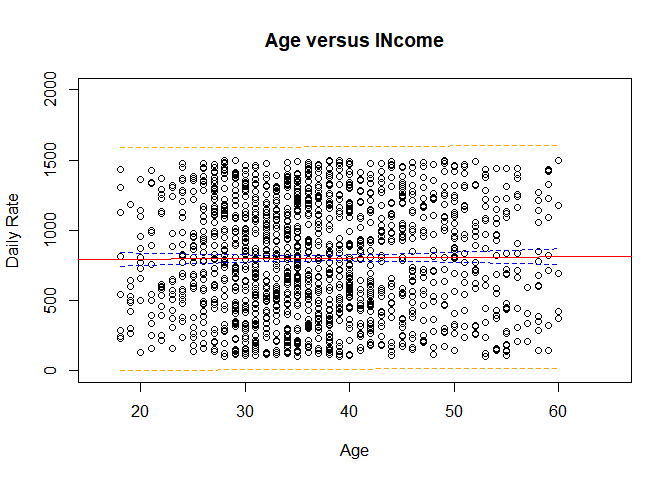
\includegraphics{DDSAnalytics_files/figure-latex/unnamed-chunk-12-1} \end{center}

\paragraph{Is there a relationship between life satisfaction and any
other
attribute?}\label{is-there-a-relationship-between-life-satisfaction-and-any-other-attribute}

\paragraph{What are the top 3 factors that lead to
attrition?}\label{what-are-the-top-3-factors-that-lead-to-attrition}

Using the Stepwise Variable selction method we have determined that the
most effective predictors of years with the company are Years with
Current Manager, Training Times Last Year, Years In CurrentRole, Years
Since Last Promotion, Number of Companies Worked, Age, Monthly Income,
Job Involvement, Percent Salary Hike and DailyRate.

These factors can be used to predict how long in years an employee will
stay with the company using a statistical formula.

We advise caution be used in decision making based on the following
variables for ethical or even legal reasons: * Gender\\
* Marital Status\\
* Relationship Satisfaction\\
* Total Working Years * Age

Our model actually only uses one of these factors (Age) which if used as
a factor in decision making could be considered discriminatory therefore
this analysis should be used with caution.

Inference can only be drawn to the employees in our dataset and not an
larger external population.

The top 3 factors that predict how long an employee will stay with the
company in years are Years With Current Manager, Training Times Last
Year and YearsInCurrentRole

Though this analysis is significant it is merely a proof of concept;
higher quality results can be achieved wiht additional time and
resources for analyzing the data.

\paragraph{Appendix}\label{appendix}

\begin{verbatim}
## Stepwise Selection Method   
## ---------------------------
## 
## Candidate Terms: 
## 
## 1. Age 
## 2. DailyRate 
## 3. DistanceFromHome 
## 4. Education 
## 5. EnvironmentSatisfaction 
## 6. HourlyRate 
## 7. JobInvolvement 
## 8. JobLevel 
## 9. JobSatisfaction 
## 10. MonthlyIncome 
## 11. MonthlyRate 
## 12. NumCompaniesWorked 
## 13. PercentSalaryHike 
## 14. PerformanceRating 
## 15. RelationshipSatisfaction 
## 16. StockOptionLevel 
## 17. TotalWorkingYears 
## 18. TrainingTimesLastYear 
## 19. WorkLifeBalance 
## 20. YearsInCurrentRole 
## 21. YearsSinceLastPromotion 
## 22. YearsWithCurrManager 
## 
## We are selecting variables based on p value...
## 
## Variables Entered/Removed: 
## 
## - YearsWithCurrManager added 
## - TrainingTimesLastYear added 
## - YearsInCurrentRole added 
## - YearsSinceLastPromotion added 
## - NumCompaniesWorked added 
## - Age added 
## - MonthlyIncome added 
## - JobInvolvement added 
## - PercentSalaryHike added 
## - DailyRate added 
## 
## No more variables to be added/removed.
## 
## 
## Final Model Output 
## ------------------
## 
##                         Model Summary                          
## --------------------------------------------------------------
## R                       0.884       RMSE                2.877 
## R-Squared               0.781       Coef. Var          41.051 
## Adj. R-Squared          0.779       MSE                 8.277 
## Pred R-Squared          0.775       MAE                 1.897 
## --------------------------------------------------------------
##  RMSE: Root Mean Square Error 
##  MSE: Mean Square Error 
##  MAE: Mean Absolute Error 
## 
##                                  ANOVA                                   
## ------------------------------------------------------------------------
##                  Sum of                                                 
##                 Squares          DF    Mean Square       F         Sig. 
## ------------------------------------------------------------------------
## Regression    43062.379          10       4306.238    520.292    0.0000 
## Residual      12075.523        1459          8.277                      
## Total         55137.902        1469                                     
## ------------------------------------------------------------------------
## 
##                                         Parameter Estimates                                          
## ----------------------------------------------------------------------------------------------------
##                   model      Beta    Std. Error    Std. Beta      t        Sig      lower     upper 
## ----------------------------------------------------------------------------------------------------
##             (Intercept)     2.117         0.563                  3.756    0.000     1.011     3.222 
##    YearsWithCurrManager     0.563         0.032        0.328    17.770    0.000     0.500     0.625 
##   TrainingTimesLastYear     0.240         0.020        0.305    12.143    0.000     0.202     0.279 
##      YearsInCurrentRole     0.468         0.032        0.277    14.780    0.000     0.406     0.530 
## YearsSinceLastPromotion     0.310         0.029        0.163    10.714    0.000     0.254     0.367 
##      NumCompaniesWorked    -0.286         0.033       -0.117    -8.769    0.000    -0.350    -0.222 
##                     Age    -0.030         0.012       -0.045    -2.589    0.010    -0.053    -0.007 
##           MonthlyIncome     0.000         0.000        0.047     2.443    0.015     0.000     0.000 
##          JobInvolvement    -0.191         0.106       -0.022    -1.807    0.071    -0.399     0.016 
##       PercentSalaryHike    -0.036         0.021       -0.021    -1.742    0.082    -0.076     0.005 
##               DailyRate     0.000         0.000       -0.021    -1.716    0.086    -0.001     0.000 
## ----------------------------------------------------------------------------------------------------
\end{verbatim}

\begin{verbatim}
## 
##                                       Stepwise Selection Summary                                        
## -------------------------------------------------------------------------------------------------------
##                                     Added/                   Adj.                                          
## Step           Variable            Removed     R-Square    R-Square      C(p)          AIC        RMSE     
## -------------------------------------------------------------------------------------------------------
##    1     YearsWithCurrManager      addition       0.592       0.591    1244.3580    8189.0915    3.9161    
##    2     TrainingTimesLastYear     addition       0.687       0.687     610.6050    7798.1456    3.4274    
##    3      YearsInCurrentRole       addition       0.744       0.744     234.6420    7504.4996    3.1005    
##    4    YearsSinceLastPromotion    addition       0.764       0.763     107.8300    7390.4311    2.9815    
##    5      NumCompaniesWorked       addition       0.777       0.777      19.5680    7305.2675    2.8954    
##    6              Age              addition       0.779       0.778      13.4860    7299.2046    2.8885    
##    7         MonthlyIncome         addition       0.780       0.779       9.2750    7294.9777    2.8833    
##    8        JobInvolvement         addition       0.780       0.779       7.8470    7293.5298    2.8810    
##    9       PercentSalaryHike       addition       0.781       0.779       6.6830    7292.3412    2.8788    
##   10           DailyRate           addition       0.781       0.779       5.7510    7291.3789    2.8769    
## -------------------------------------------------------------------------------------------------------
\end{verbatim}

\begin{verbatim}
## 
## Call:
## lm(formula = YearsAtCompany ~ YearsWithCurrManager + TrainingTimesLastYear + 
##     YearsInCurrentRole + YearsSinceLastPromotion + NumCompaniesWorked + 
##     Age + MonthlyIncome + JobInvolvement + PercentSalaryHike + 
##     DailyRate, data = MyPredictionData)
## 
## Coefficients:
##             (Intercept)     YearsWithCurrManager    TrainingTimesLastYear  
##               2.117e+00                5.626e-01                2.404e-01  
##      YearsInCurrentRole  YearsSinceLastPromotion       NumCompaniesWorked  
##               4.678e-01                3.104e-01               -2.857e-01  
##                     Age            MonthlyIncome           JobInvolvement  
##              -2.995e-02                6.177e-05               -1.914e-01  
##       PercentSalaryHike                DailyRate  
##              -3.578e-02               -3.204e-04
\end{verbatim}

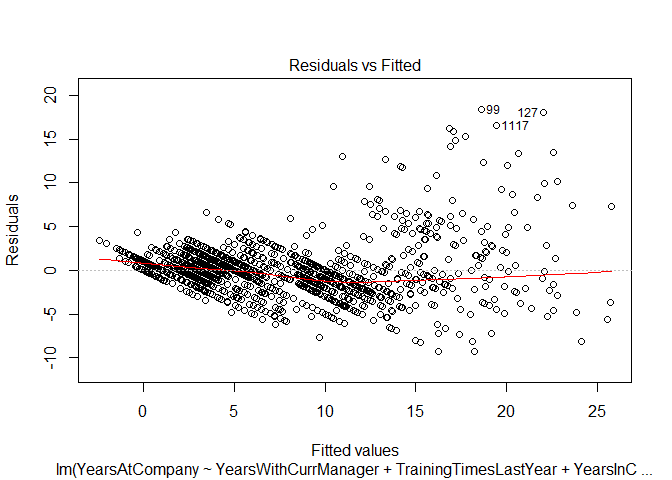
\includegraphics{DDSAnalytics_files/figure-latex/unnamed-chunk-17-1.pdf}
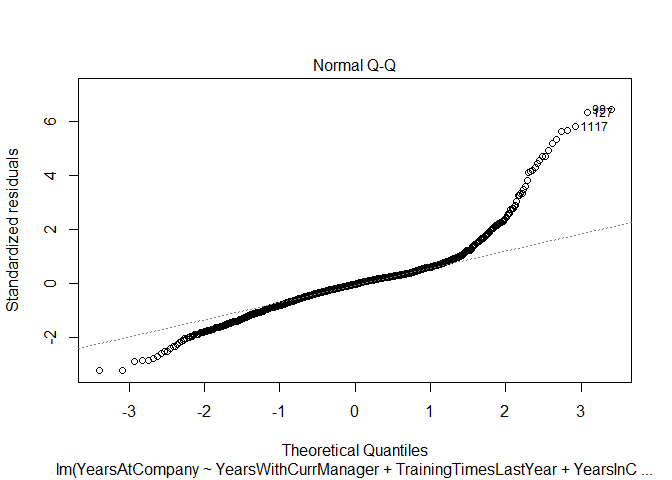
\includegraphics{DDSAnalytics_files/figure-latex/unnamed-chunk-17-2.pdf}
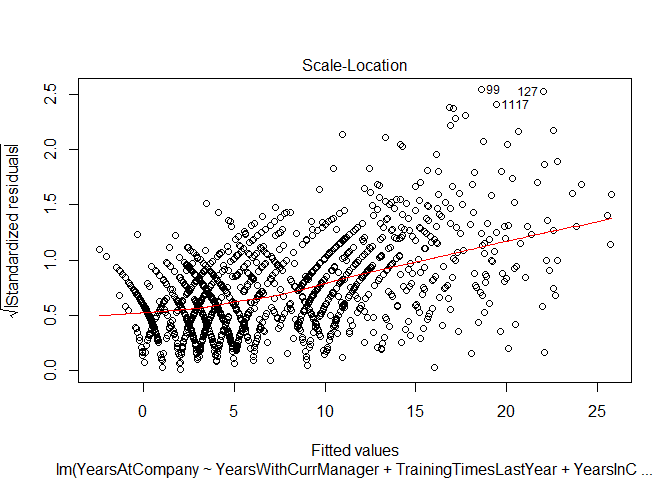
\includegraphics{DDSAnalytics_files/figure-latex/unnamed-chunk-17-3.pdf}
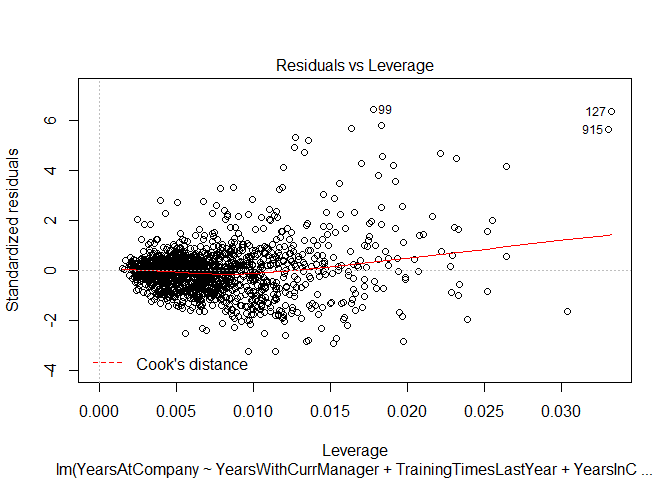
\includegraphics{DDSAnalytics_files/figure-latex/unnamed-chunk-17-4.pdf}


\end{document}
